\section{Application 3: Systematic Analysis}
\label{sec:app_err_analysis}


\begin{figure}[t]
\centering
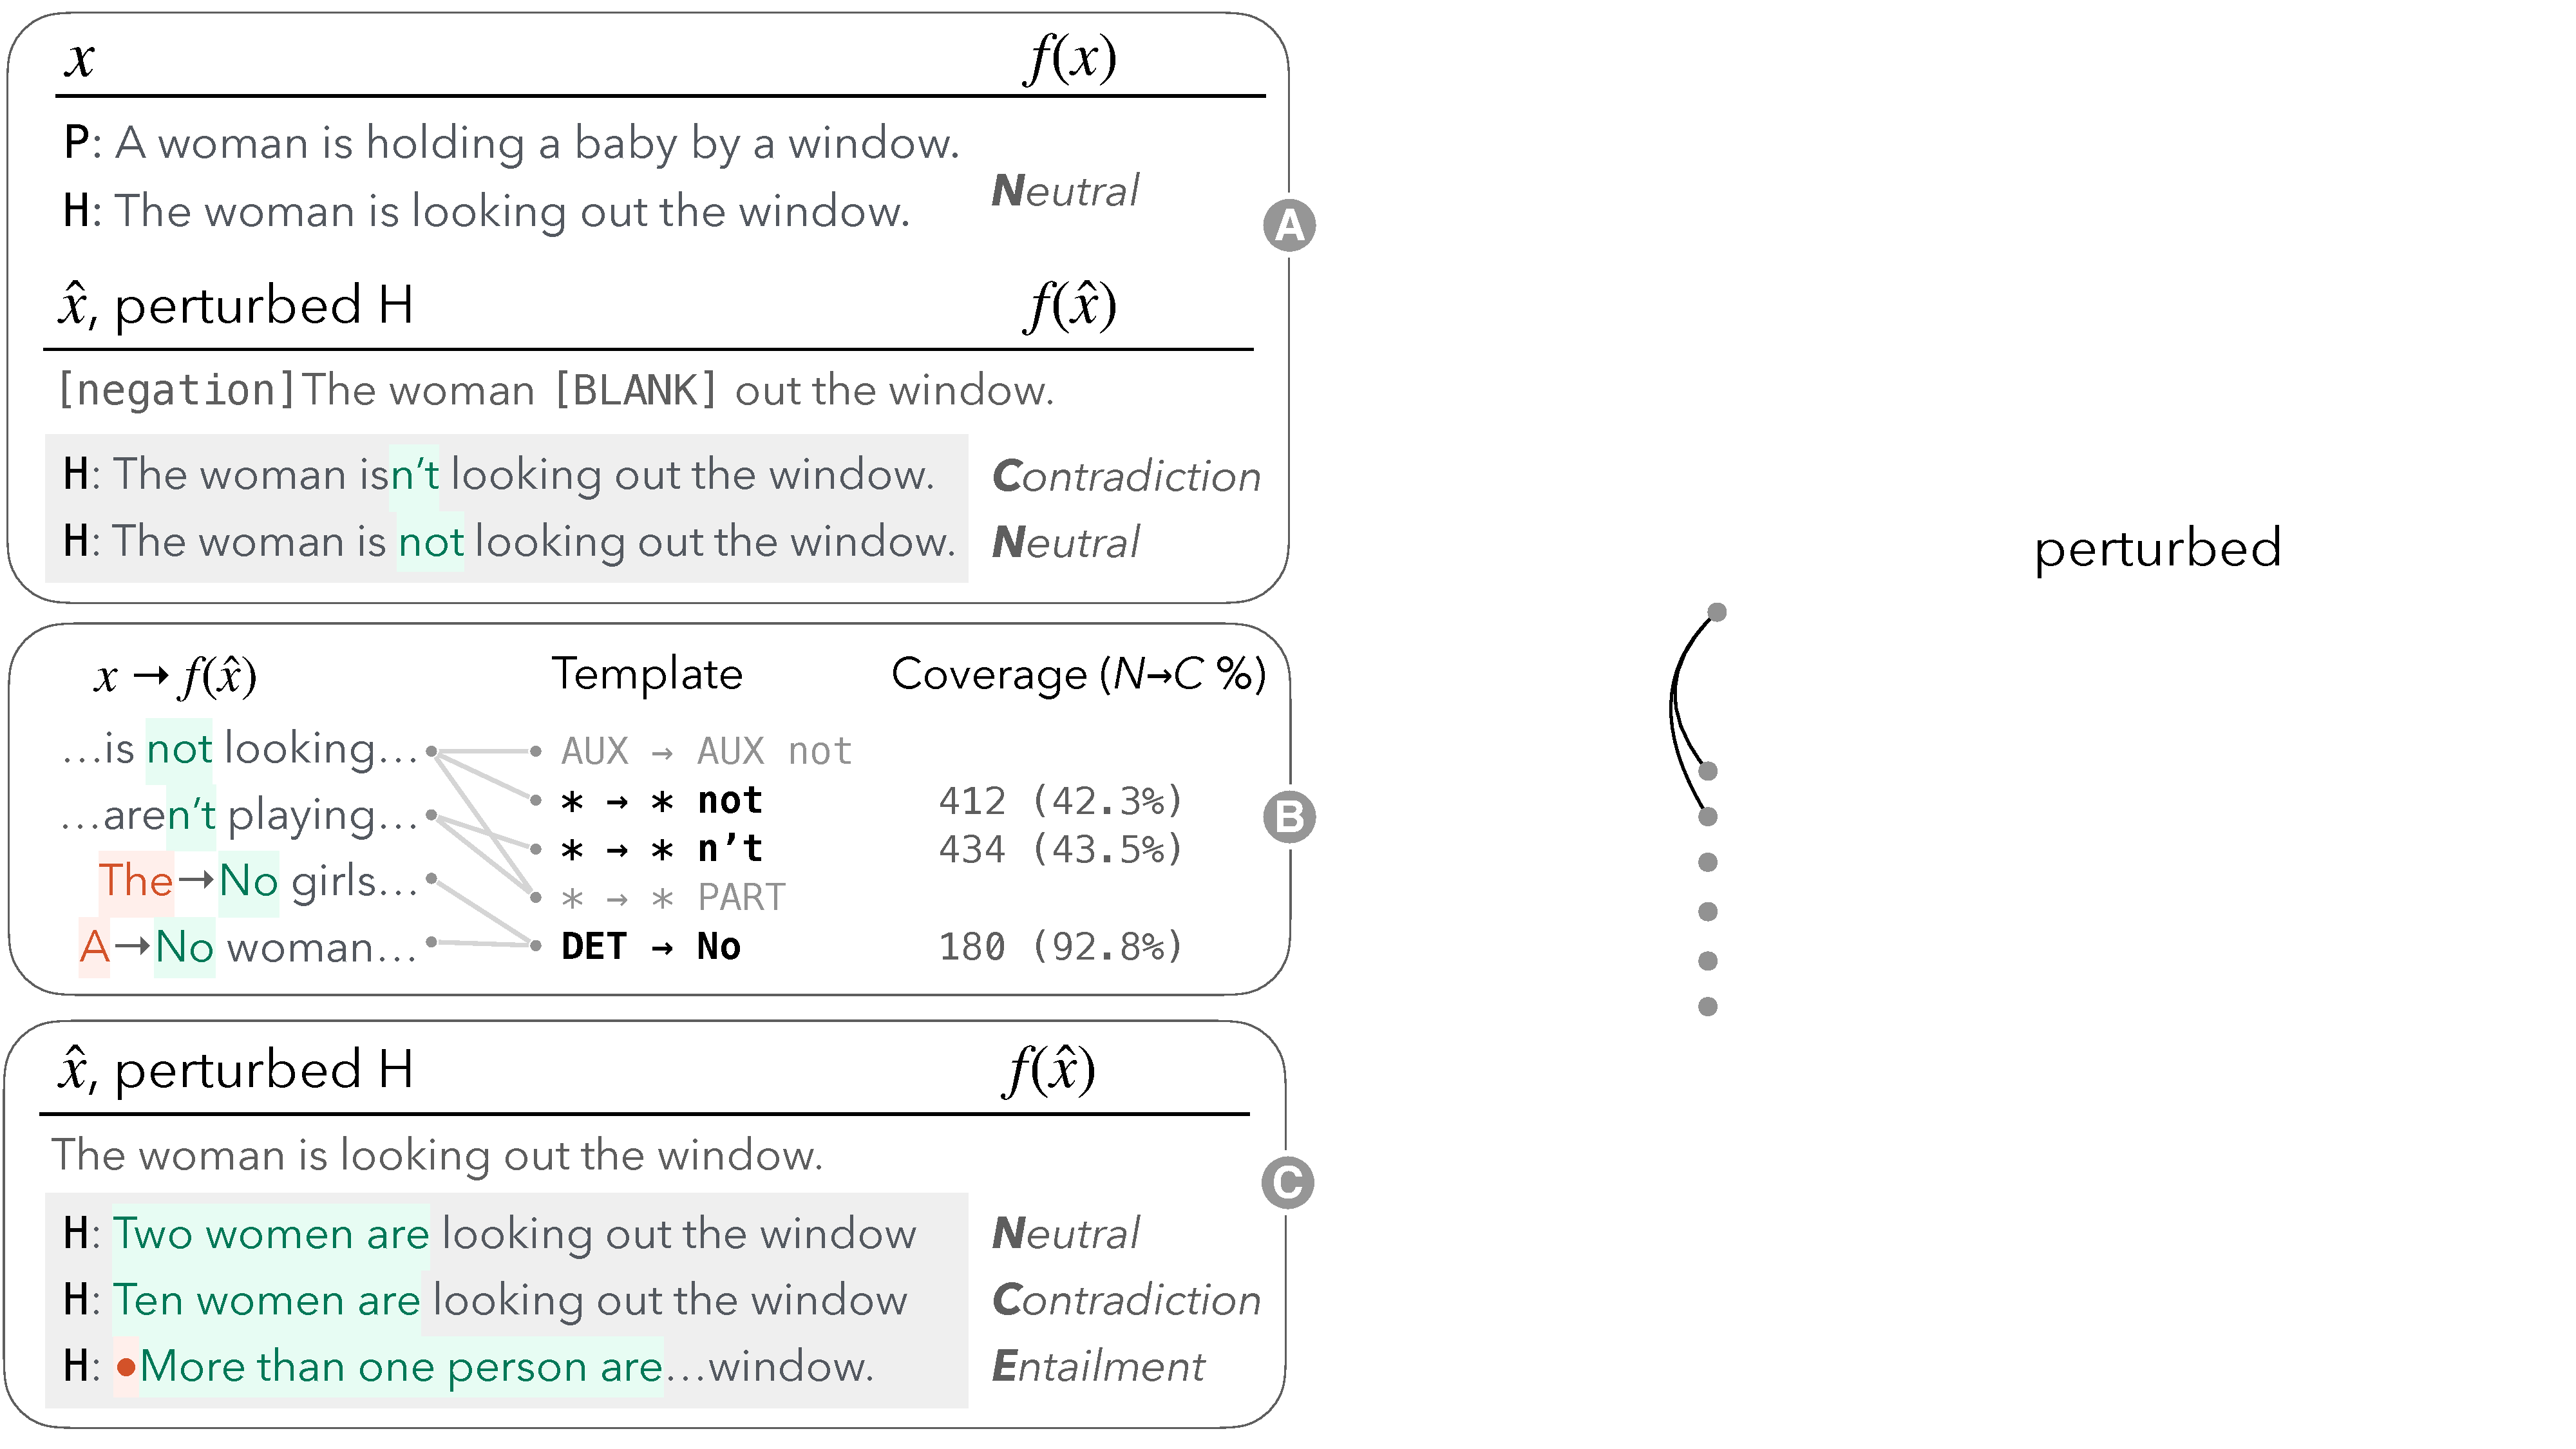
\includegraphics[trim={0 1cm 33cm 0cm},clip,width=1\columnwidth]{figures/err_analysis.pdf}
\vspace{-15pt}
\caption{
(A) A \nli case with a correct \emph{Neutral} prediction.
Through strict \tagstrs and blanks shown in the figure, \sysname generates two $\xp$ that negate the hypothesis sentence \emph{H}, which result in different predictions.
(B) By extracting and selecting representative templates from different $\xp$, we can systematically compare a model's response to certain perturbation patterns, \eg the model flips to predict \emph{Contradiction} much more on \swap{\texttt{DET}}{no}.
(C) Another blank placement that leads to analyses on \emph{quantifiers}.
}
\vspace{-10pt}
\label{fig:err_analysis}
\end{figure}


Previous applications focus on a selected subset of $\xp$, but the access to the entire pool is also important.
Through a case study on the \nli RoBERTa model in \S\ref{subsec:contrast_set}, we demonstrate that \sysname's ability to generate \emph{multiple} counterfactuals per $x$ is essential for systematic error analysis~\cite{wu2019errudite}.
Here, the generation is largely driven by human analysts, and the relationship $\relation{\xp}$ can be determined by human domain expertise.


\emph{Form model behavior hypotheses by inspecting counterfactuals around one instance.}
\citet{gururangan2018annotation} asserted that negation is correlated with the class label \emph{contradiction}. 
To verify it, we can randomly select a \emph{neutral} instance $x$ as in Figure~\ref{fig:err_analysis}A, and inspect its counterfactuals that \emph{only} negate the hypothesis sentence.
\sysname produces two $\xp$:
While \exinline{is\add{n't}} seems to confirm the overfit to negation, \exinline{is not} shows a counterexample. 
We therefore hypothesize: 
\emph{The model has more nuanced responses to different kinds of negations}, overfitting to some patterns more than others.

\emph{Verify the hypothesis through systematic counterfactual analysis.}
To verify that the hypothesis generalizes beyond one instance, we compare the impact of different negation patterns on \emph{a group of} 895 original examples that have \emph{neutral} groundtruths and predictions.
For each $x$, we collect multiple counterfactuals that negate the hypothesis through the \ctrltag{negation} code.
Then, similar to \citet{wu2020tempura}, we select representative negation patterns.
As shown in Figure~\ref{fig:err_analysis}B, we extract \emph{templates} from each $\xp$ by abstracting the modified spans into different combinations of linguistic features, and select the templates that cover various counterfactuals through weighted set coverage (details in Appendix~\ref{appendix:err_analysis_template}).
The top three templates selected (in bold) show interesting contrasts:
First, counter to our observation on Figure~\ref{fig:err_analysis}A, the model is relatively stable on \add{not} and \add{n't} --- they both around 43\% \emph{neutral} predictions to \emph{contradiction}, while maintaining others.
However, the model does responds much more aggressively to \swap{\texttt{DET}}{no}, partially confirming our hypothesis.

\emph{Drill-down through interactive blanking.}
If \add{not} and \add{n't} are generally stable, what causes the difference in Figure~\ref{fig:err_analysis}A?
We can drill down add blanks to the negated hypothesis.
For example, inspired by the returns from \exinline{\texttt{[BLANK]} is\add{n't}/\add{not} looking out the window.}, we find changing \swap{woman} to \add{girl}, \add{boy}, and \add{man} in both the \emph{P} and the \emph{H} would all eliminate the difference, whereas \add{person} cannot.
Intrigued by the impact of subjects, we also apply a similar blanking to the original \emph{H}.
The wild predictions in Figure~\ref{fig:err_analysis}C lead us to further hypothesize that the model does not understanding quantifiers, which we verify in Appendix~\ref{appendix:err_analysis_quantifier_case}.


\paragraph{Takeaways.}
The case highlights unique benefits from \sysname.
First, the \emph{over-} generation helps analysts contrast similar perturbations, and form hypotheses that can be missed otherwise.
Human analysts rarely check both \swap{is}{is not} and \swap{is}{isn't}, and therefore can hardly realize they can be on different sides of the decision boundary --- echoing our observation in \S\ref{subsec:exp_user_study} that human counterfactual analysis may be incomplete and misleading.

Moreover, driven by the \tagstrs, \sysname allows inspecting patterns that are hard to retrieve from existing masked language models.
When applying RoBERTa to the same blanked (masked) hypotheses, we obtain less than 5\% counterfactuals were related to negation compared to the \sysname ones.
Instead, more than 1000 counterfactuals are related to \texttt{\swap{is}{VERB}} and \texttt{\swap{are}{VERB}}.
Similarly, RoBERTa would not be able to produce examples in Figure~\ref{fig:err_analysis}C, as it focuses on single word replacement.
The apparent gap shows that the use of control code is promising for interactive and targeted generation.

%Moreover, with \sysname diversifying the text chunks to change, it \sysname helps contrast similar changes that happen at different places.
%While \sysname enables the comparison between \swap{\texttt{VERB}}{\texttt{not VERB}} and \swap{\texttt{DET}}{no}, RoBERTa focus on changing \texttt{VERB}: the top two templates from it are \texttt{\swap{is}{VERB}} and \texttt{\swap{are}{VERB}}, producing 1000 conterfactuals in total.